\chapter{Sobolev en la recta real}

\textbf{Ejemplo 1.}
$\langle p(t),q(t) \rangle_{\textbf{M}_S}=\int_{-1}^{1} p(t)q(t)t^2 \, dt + \int_{-1}^{1} p'(t)q'(t)t^{10} \, dt $

\begin{center}
	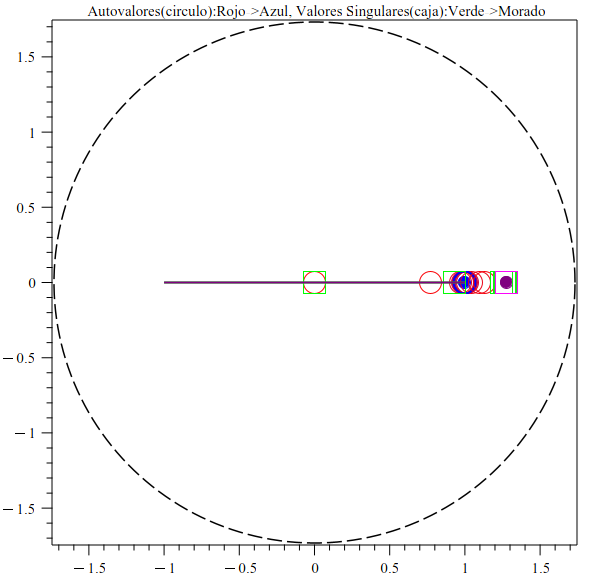
\includegraphics[width=0.9\textwidth]{include/a-1b1t2t10.png}
\end{center}

Observamos que $\lim_{n \to 50}\|\mathcal{D}_{n}\|=1.276$ acota a $Z_{50}=\{t\in\mathbb{R}: \exists n \in \{1,...,50\},\varphi_n(t)=0\}$. Tenemos que $\max\{Z_{n}\}_{n=0}^{50}=1.133$ pero $\lim_{n \to 50} \max{Z_{n}} = 0.999 $, observamos que los ceros convergen al límite del soporte.

\textbf{Ejemplo 2.}
$\langle p(t),q(t) \rangle_{\textbf{M}_S}=\int_{-1}^{1} p(t)q(t)t^{10} \, dt + \int_{-1}^{1} p'(t)q'(t)t^{2} \, dt $

\begin{center}
	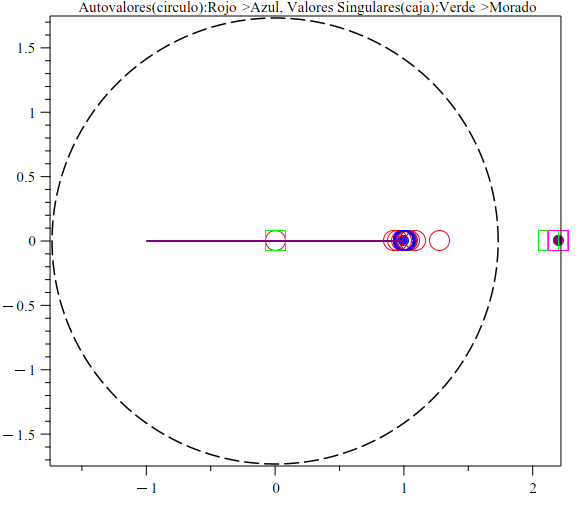
\includegraphics[width=0.9\textwidth]{include/a-1b1t10t2.png}
\end{center}

Este ejemplo no es secuencialmente dominado pero aun así los ceros están acotados y dentro del disco $D(0,\sqrt{3})$. De hecho en este caso $\lim_{n \to 50}\|\mathcal{D}_{n}\|=2.204$ tambien está acotado, $\lim_{n \to 50} \max{Z_{n}} = 0.999 $ y $\max\{Z_{n}\}_{n=0}^{50}=1.275$.

Cuando $[c,d] \nsubseteq [a,b]$ entonces no podemos hablar de secuencialmente dominados. En este caso veremos el resultado de M. Alfaro y M. Luisa Rezola.

\textbf{Teorema 2.} Si co($S_{\mu_0}$) $\cap$ co($S_{\mu_1}$) = $\emptyset$, entonces los ceros de $Q'_n$ son simples
y están contenidos en el interior de co($S_{\mu_0}$) $\cup$ co($S_{\mu_1}$), y los ceros de $Q_n$ están
contenidos en el disco centrado en el punto de co($S_{\mu_1}$) más alejado de co($S_{\mu_0}$) y
radio el diámetro de co($S_{\mu_0}$) $\cup$ co($S_{\mu_1}$).\todo{me gustaria tener la demostración}

\textbf{Ejemplo 3.}
$\langle p(t),q(t) \rangle_{\textbf{M}_S}=\int_{0}^{10} p(t)q(t) \, dt + \int_{30}^{40} p'(t)q'(t) \, dt $

\begin{center}
	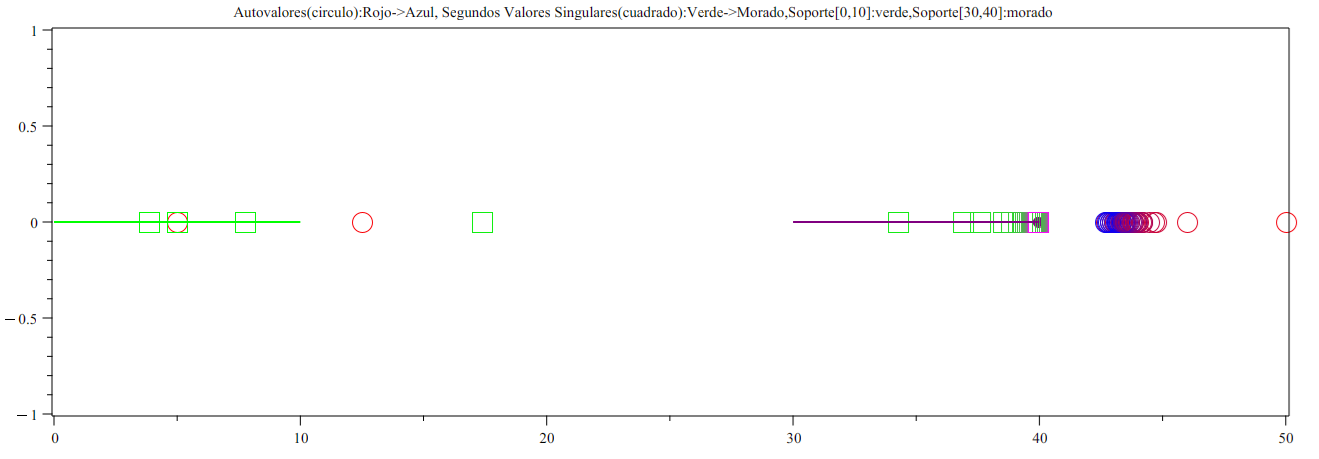
\includegraphics[width=1\textwidth]{include/a0b10c30d40.png}
\end{center}

En este ejemplo no se han mostrado los valores singulares máximos ya que tienden a infinito, por lo que no podemos usar como cota $\|\mathcal{D}\|$, sin embargo podemos observar que los ceros si están acotados, que $\lim_{n \to 50} \max{Z_{n}} = 43.133$ y que $\max\{Z_{n}\}_{n=0}^{50}=50.052$. Es interesante ver que convergen fuera del soporte y que el segundo mayor valor singular de $\mathcal{D}_{50}=39.975$, por lo que en lugar de usar la norma de $\mathcal{D}$, podemos considerar este valor singular para acotar, esta idea se continuará en los siguientes ejemplos ya que $\mathcal{D}$ no estará acotada.

\textbf{Ejemplo 4.}
$\langle p(t),q(t) \rangle_{\textbf{M}_S}=\int_{30}^{40} p(t)q(t) \, dt + \int_{0}^{10} p'(t)q'(t) \, dt $

\begin{center}
	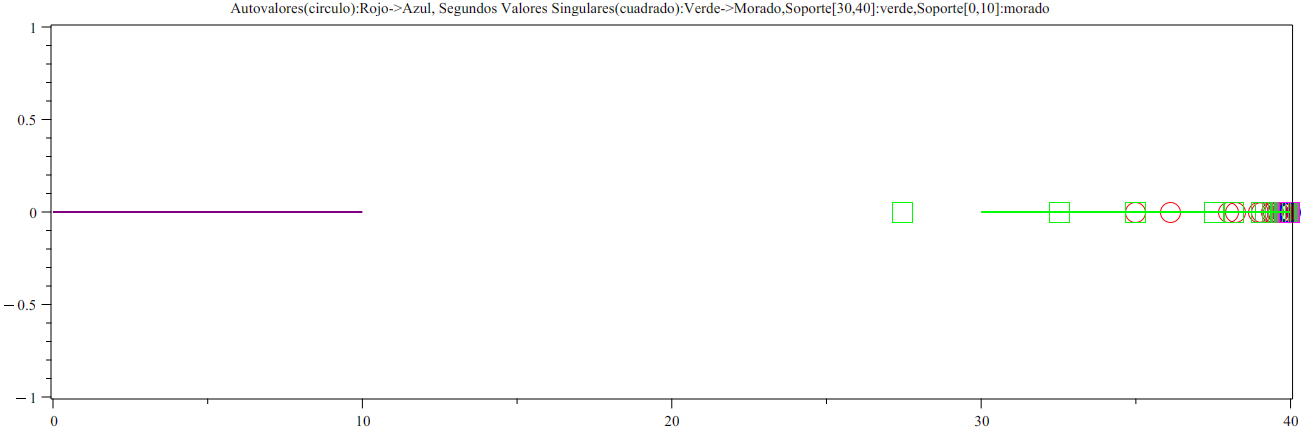
\includegraphics[width=1\textwidth]{include/a30b40c0d10.png}
\end{center}

Comparando este ejemplo con el anterior podemos ver que la derivada afecta a la convergencia de los ceros, ya que en este podemos observar como convergen al límite del soporte, $\lim_{n \to 50}{\max{Z_n}}=\max\{Z_{n}\}_{n=0}^{50}=39.983$. Como en el ejemplo anterior, $\|\mathcal{D}\|$ no está acotada y vemos que el segundo mayor valor singular de converge a $\mathcal{D}_{50}=39.982$ por lo que parece un buen candidato para usar como cota.

\textbf{Ejemplo 5.}
$\langle p(t),q(t) \rangle_{\textbf{M}_S}=\int_{0}^{10} p(t)q(t) \, dt + \int_{30}^{50} p'(t)q'(t) \, dt $

\begin{center}
	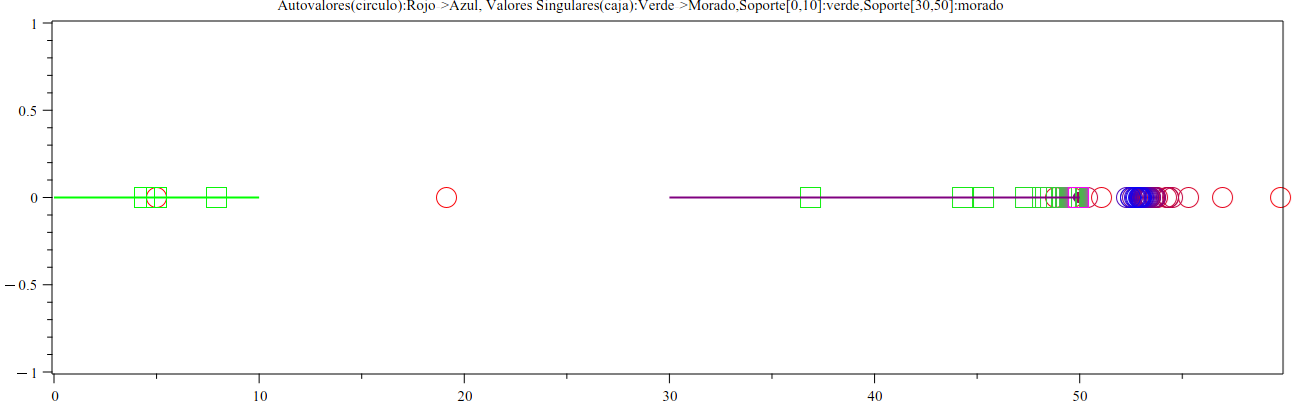
\includegraphics[width=1\textwidth]{include/a0b10c30d50.png}
\end{center}

Para este ejemplo el segundo soporte es más grande, pero la distancia entre soportes sigue igual. Podemos observar que los ceros convergen $\lim_{n \to 50} \max{Z_n}=52.763$ y $\max\{Z_{n}\}_{n=0}^{50}=59.814$. Continuamos con $\|\mathcal{D}\|$ no acotada y el segundo mayor valor singular de $\mathcal{D}_{50}=49.966$. Es interesante observar que la distancia entre el soporte y la convergencia de los ceros se mantiene similar, solo se ha desplazado la misma distancia que ha crecido el soporte.

\textbf{Ejemplo 6.}
$\langle p(t),q(t) \rangle_{\textbf{M}_S}=\int_{30}^{50} p(t)q(t) \, dt + \int_{0}^{10} p'(t)q'(t) \, dt $

\begin{center}
	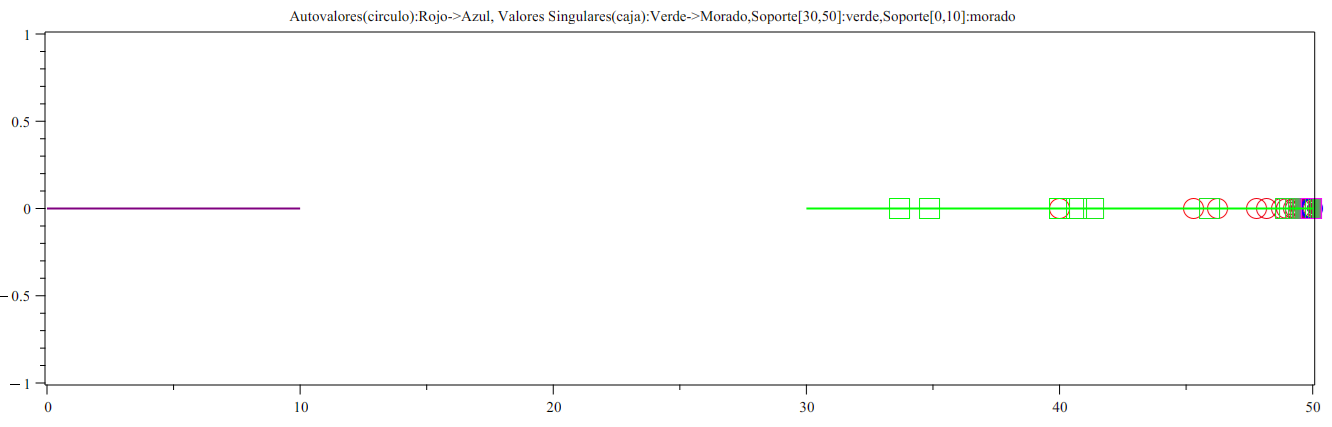
\includegraphics[width=1\textwidth]{include/a30b50c0d10.png}
\end{center}

En este caso $\lim_{n \to 50} \max{Z_n}=\max\{Z_{n}\}_{n=0}^{50}=49.975$. La norma de $\mathcal{D}$ no está acotada y el segundo mayor valor singular de $\mathcal{D}_{50}=49.975$.

\textbf{Ejemplo 7.}
$\langle p(t),q(t) \rangle_{\textbf{M}_S}=\int_{0}^{20} p(t)q(t) \, dt + \int_{30}^{40} p'(t)q'(t) \, dt $

\begin{center}
	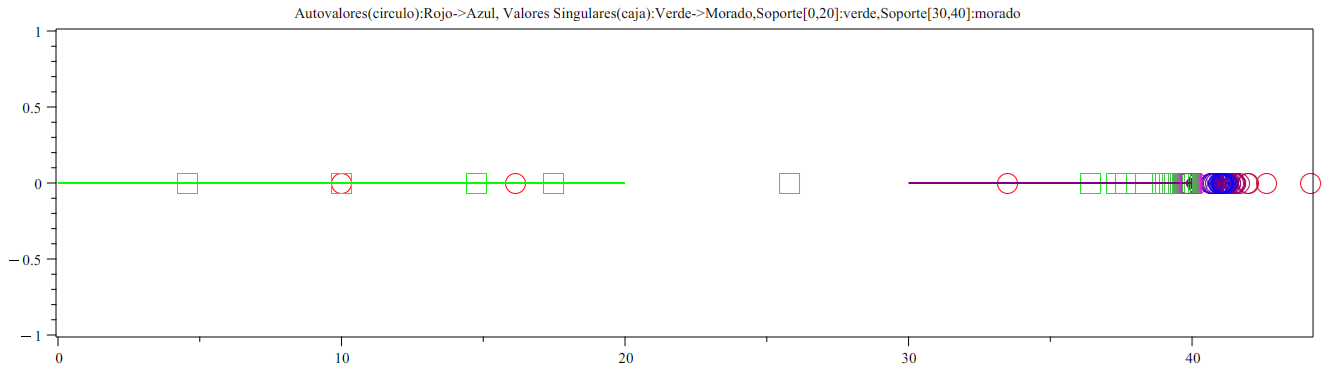
\includegraphics[width=1\textwidth]{include/a0b20c30d40.png}
\end{center}

Se puede observar como se mantiene la conjetura cuando se da el caso contrario, ya que los ceros convergen fuera del soporte proporcional a la distancia entre soportes, $\lim_{n \to 50} \max{Z_n}=41.066$ y $\max\{Z_{n}\}_{n=0}^{50}=44.196$. La norma de $\mathcal{D}$ no está acotada y el segundo mayor valor singular de $\mathcal{D}_{50}=39.970$.

\textbf{Ejemplo 8.}
$\langle p(t),q(t) \rangle_{\textbf{M}_S}=\int_{30}^{40} p(t)q(t) \, dt + \int_{0}^{20} p'(t)q'(t) \, dt $

\begin{center}
	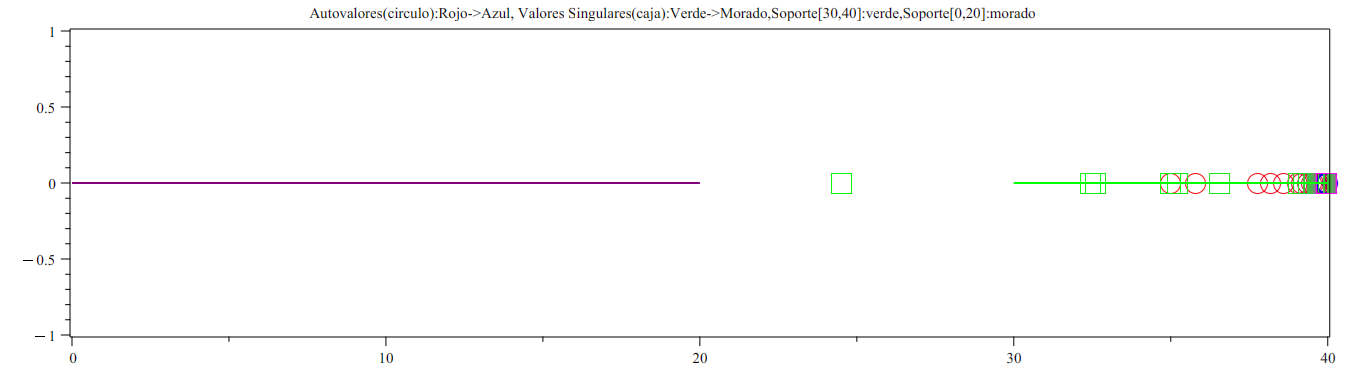
\includegraphics[width=1\textwidth]{include/a30b40c0d20.png}
\end{center}

En este ejemplo los ceros convergen al límite del soporte, $\lim_{n \to 50} \max{Z_n}=\max\{Z_{n}\}_{n=0}^{50}=39.979$. La norma de $\mathcal{D}$ no está acotada y el segundo mayor valor singular de $\mathcal{D}_{50}=39.979$.

\textbf{Ejemplo 9.}
$\langle p(t),q(t) \rangle_{\textbf{M}_S}=\int_{-15}^{-5} p(t)q(t) \, dt + \int_{5}^{16} p'(t)q'(t) \, dt $

\begin{center}
	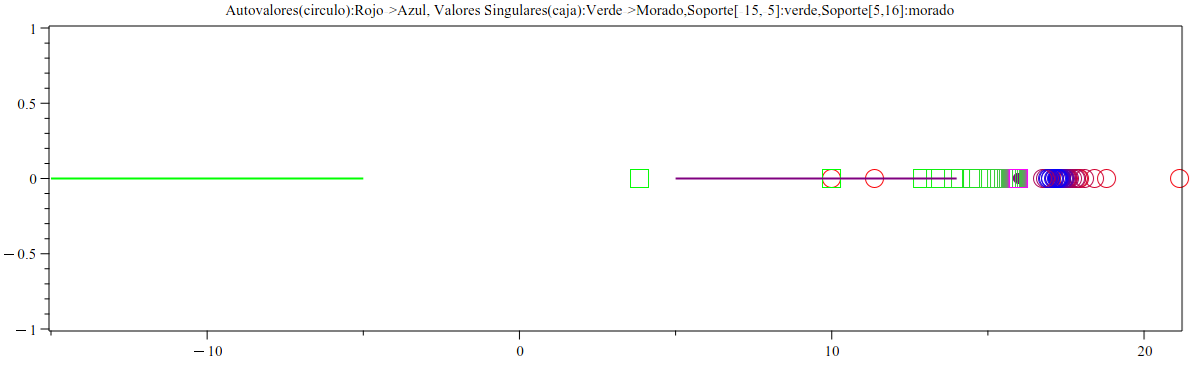
\includegraphics[width=1\textwidth]{include/a-15b-5c5d16.png}
\end{center}

Podemos observar que $\lim_{n \to 50} \max{Z_n}=17.104$ y $\max\{Z_{n}\}_{n=0}^{50}=21.152$. La norma de $\mathcal{D}$ no está acotada y el segundo mayor valor singular de $\mathcal{D}_{50}=15.980$.

\textbf{Ejemplo 10.}
$\langle p(t),q(t) \rangle_{\textbf{M}_S}=\int_{-15}^{-5} p(t)q(t) \, dt + \int_{5}^{14} p'(t)q'(t) \, dt $

\begin{center}
	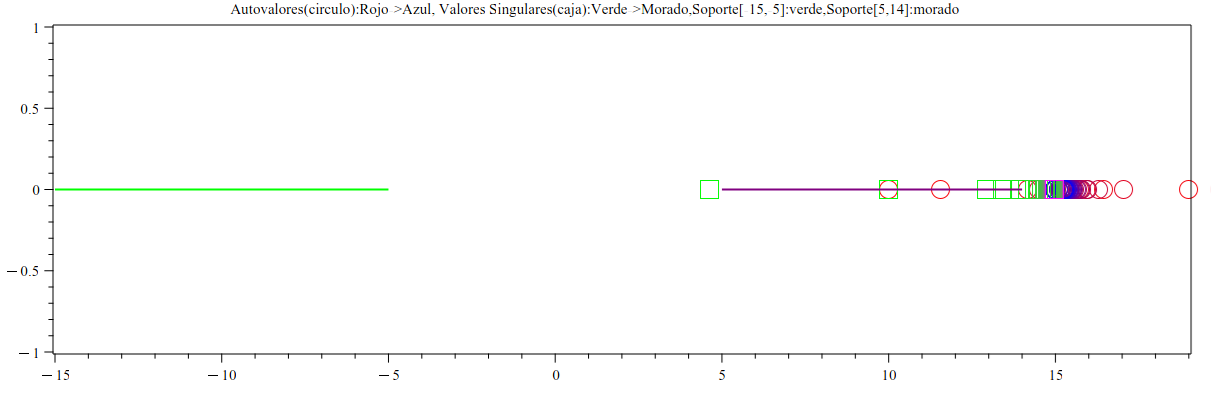
\includegraphics[width=1\textwidth]{include/a-15b-5c5d14.png}
\end{center}

En este ejemplo los ceros convergen al límite del soporte, $\lim_{n \to 50} \max{Z_n}=15.005$ y $\max\{Z_{n}\}_{n=0}^{50}=19.007$. La norma de $\mathcal{D}$ no está acotada y el segundo mayor valor singular de $\mathcal{D}_{50}=14.985$.

Tras ver todos los ejemplos podemos conjeturar lo siguiente:\todo{lo que es claro es que lo que suceda con los soportes influye mucho, ya sea tamaño, extremos o intersección.}
\begin{itemize}
	\item El segundo mayor valor singular de $\mathcal{D}_{n}$ converge al extremo con mayor módulo de los soportes. Se puede encontrar una constante de proporción o de desviacion $K$ que depende de los soportes (extremos,intersección, tamaño) para poder acotar los ceros.\todo{puede que la k y K esten relacionadas}
	\item $\lim_{n \to \infty} \max{Z_n}=\max\{|a|,|b|,|c|,|d|\} + k = \max\{|a|,|b|,|c|,|d|\} \cdot k'$
	\item El $k$ cuando $\max\{|a|,|b|\} < \max\{|c|,|d|\}$ es notablemente mayor que el $k$ cuando ocurre lo contrario.
	\item $k$ o $k'$ depende de la posición relativa entre los soportes.
	      \begin{itemize}
		      \item Si $[a,b] \cap [c,d] = \emptyset$ y $dist(b,c) < dist(a,b) + dist(c,d)$ entonces $k$ o $k'$ no crece mucho.
		      \item Si $[a,b] \cap [c,d] = \emptyset$ y $dist(b,c) > dist(a,b) + dist(c,d)$ entonces $k$ o $k'$ crece mucho.
		      \item Si $[a,b] \cap [c,d] \neq \emptyset$ entonces $k$ o $k'$ crece muy poco. Mientras mayor sea $dist(b,c)$ menos crece $k$ o $k'$.
	      \end{itemize}
\end{itemize}
\todo{Tengo que hacer mas pruebas porque con tantos casos termina confundiendo que es lo que pasa.}

Dejando de lado los productos de Sobolev, consideremos el producto interno de la forma:
$$\langle p(t),q(t) \rangle = \int_{a}^{b} p(t) q(t) \, dt + |p'(c)||q'(c)|.$$
Este producto interno es muy interesante ya que solo introduce un átomo al producto interno usual, y sin embargo el operador multiplicación no es acotado. En los siguientes ejemplos se mostrará que los ceros de los polinomios ortogonales asociados a este producto interno están acotados, y que podemos encontrar una cota.

\textbf{Ejemplo 11.} $\langle p(t),q(t) \rangle = \int_{-1}^{1} p(t) q(t) \, dt + |p'(0)||q'(0)|.$

\begin{center}
	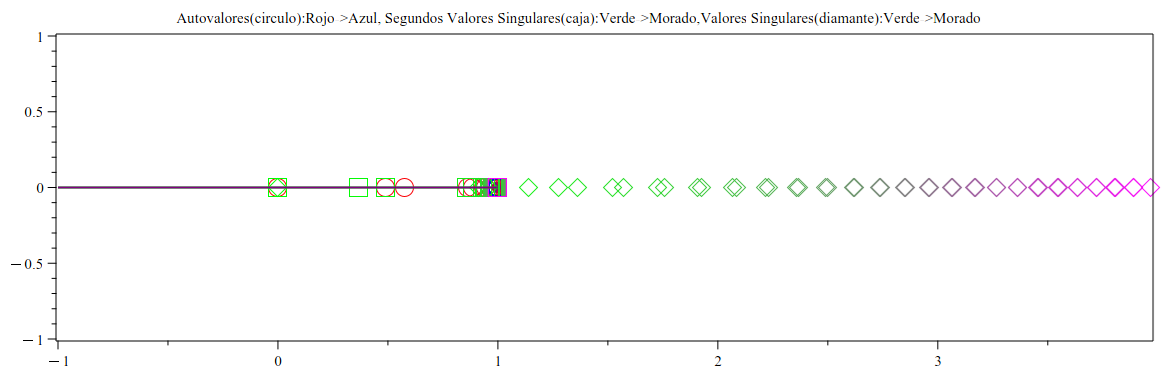
\includegraphics[width=1\textwidth]{include/a-1b1t0.png}
\end{center}

En este ejemplo podemos observar que los ceros convergen al límite del soporte, $\lim_{n \to 50} \max{Z_n}=\max\{Z_{n}\}_{n=0}^{50}=0.999$. La norma de $\mathcal{D}$ no está acotada, pero no es como en los casos anteriores que rápidamente se iba a infinito, en esta caso para $\mathcal{D}_{50}=3.971$ se observa que a partir de un $n_0$ hace incrementos constantes, y el segundo mayor valor singular de $\mathcal{D}_{50}=0.999$, el cual parece ser una buena cota para los ceros.

\textbf{Ejemplo 12.} $\langle p(t),q(t) \rangle = \int_{-1}^{1} p(t) q(t) \, dt + |p'(2)||q'(2)|.$

\begin{center}
	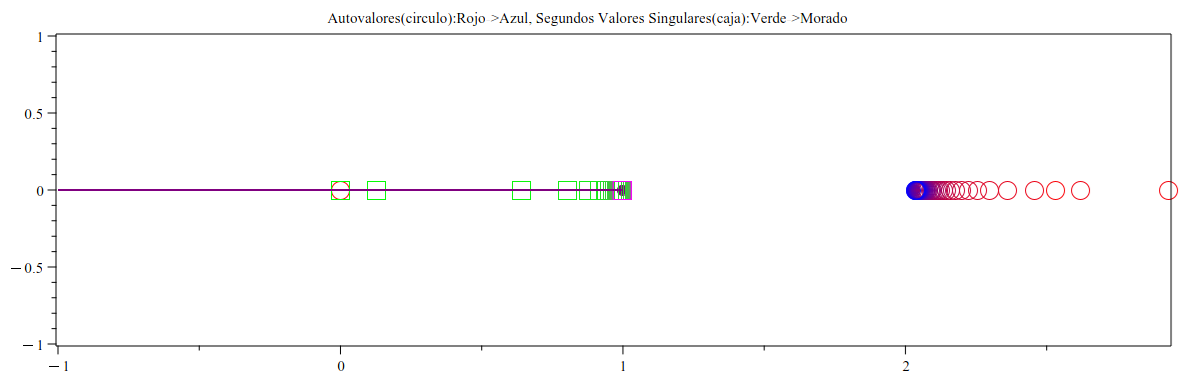
\includegraphics[width=1\textwidth]{include/a-1b1t2.png}
\end{center}

Para este ejemplo podemos observar como los ceros convergen al átomo y no al límite del soporte, $\lim_{n \to 50} \max{Z_n}=2.0356$ y $\max\{Z_{n}\}_{n=0}^{50}=2.933$. La norma de $\mathcal{D}$ no está acotada y en este caso si se va a infinito rápidamente, y el segundo mayor valor singular de $\mathcal{D}_{50}=1.999$, como en todos los casos anteriores el segundo mayor valor singular converge al mayor módulo de los extremos del soporte. En este caso podemos usar el átomo como cota, aunque falta por determinar el coeficiente $k$ que se mencionaba antes para poder abarcar todos los ceros.

\textbf{Ejemplo 13.} $\langle p(t),q(t) \rangle = \int_{0}^{1} p(t) q(t) \, dt + |p'(0)||q'(0)|.$

\begin{center}
	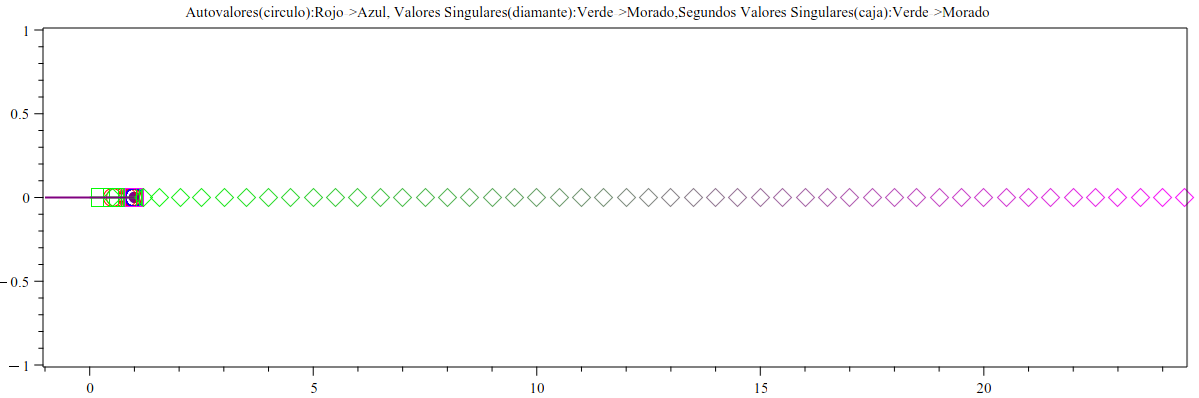
\includegraphics[width=1\textwidth]{include/a0b1t0.png}
\end{center}

En este ejemplo podemos observar que los ceros convergen al límite del soporte, $\lim_{n \to 50} \max{Z_n}=\max\{Z_{n}\}_{n=0}^{50}=0.999$. La norma de $\mathcal{D}$ no está acotada, siendo $\mathcal{D}_{50}=25.000$ y sucede como en el Ejemplo 11 que va incrementando a ritmo constante, y el segundo mayor valor singular de $\mathcal{D}_{50}=0.999$, como en todos los casos anteriores el segundo mayor valor singular converge al mayor módulo de los extremos del soporte. En este caso podemos usar el segundo mayor valor singular como cota.

\textbf{Ejemplo 14.} $\langle p(t),q(t) \rangle = \int_{0}^{1} p(t) q(t) \, dt + |p'(2)||q'(2)|.$

\begin{center}
	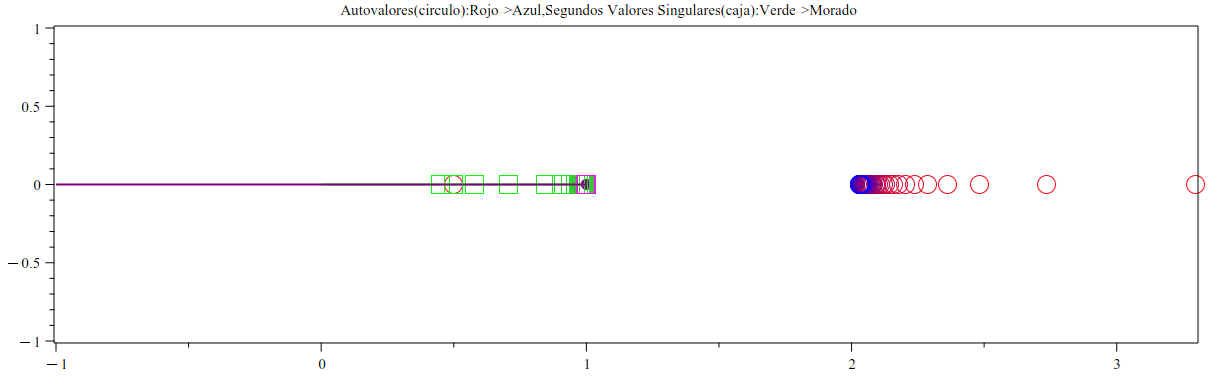
\includegraphics[width=1\textwidth]{include/a0b1t2.png}
\end{center}

En este ejemplos podemos observar que los ceros convergen al átomo y no al límite del soporte, como en el Ejemplo 12, $\lim_{n \to 50} \max{Z_n}=2.029$ y $\max\{Z_{n}\}_{n=0}^{50}=3.299$. La norma de $\mathcal{D}$ no está acotada y en este caso si se va a infinito rápidamente, y el segundo mayor valor singular de $\mathcal{D}_{50}=0.999$, como en todos los casos anteriores el segundo mayor valor singular converge al mayor módulo de los extremos del soporte. En este caso podemos usar el átomo como cota, aunque falta por determinar el coeficiente $k$ que se mencionaba antes para poder abarcar todos los ceros.

A raíz de estos ejemplos podemos conjeturar lo siguiente:

\begin{itemize}
	\item Si $c \in [a,b]$ entonces los ceros convergen al límite del soporte, y podemos usar el segundo mayor valor singular como cota.
	\item Si $c \notin [a,b]$ entonces los ceros convergen al átomo, y podemos usar el átomo como cota. Pero necesitamos determinar el coeficiente $k$ para poder abarcar todos los ceros.\todo{intuyo que tambien va a tener que ver con la posición relativa entre el soporte y el átomo, y posiblemente el tamaño del soporte.}
\end{itemize}